%%%%%%%%%%%%%%%%%%%%%%%%%%%%%%%%%%%%%%%%%%%%%%%%%%%%%%%%%%%%%%%%%%%%%%%%%%%%%%%%
% Extended abstract for the Workshop on the Future of Construction Robots.
% Target length: 3-4 pages including references.
%
% NOTE ON REFERENCES: every entry below is a real, well-known work, but the
% volume/page/year details were written from memory and must be checked against
% the publisher before submission.
%%%%%%%%%%%%%%%%%%%%%%%%%%%%%%%%%%%%%%%%%%%%%%%%%%%%%%%%%%%%%%%%%%%%%%%%%%%%%%%%

\documentclass[letterpaper, 10 pt, conference]{ieeeconf}

\IEEEoverridecommandlockouts
\overrideIEEEmargins

\usepackage{graphicx}
\usepackage{amsmath}
\usepackage{amssymb}
\usepackage{booktabs}
\usepackage{url}

\DeclareMathOperator*{\argmax}{arg\,max}

\title{\LARGE \bf
DeltaSeek: Toward Active Perception in\\Evolving Construction Environments
}

\author{Sanjay Acharjee$^{1}$ and Md Nazmus Sakib$^{2*}$% <-this % stops a space
\thanks{$^{1}$S. Acharjee is a Ph.D. Student with the Department of Civil
Engineering, University of Texas at Arlington, Arlington, TX 76019, USA
{\tt\small abirkhan.ratul@uta.edu}}%
\thanks{$^{2}$M. N. Sakib is an Assistant Professor with the Department of
Civil Engineering, University of Texas at Arlington, Arlington, TX 76019, USA
{\tt\small mdnazmus.sakib@uta.edu}}%
\thanks{$^{*}$Corresponding author: M. N. Sakib.}%
}

\begin{document}

\maketitle
\thispagestyle{empty}
\pagestyle{empty}

%%%%%%%%%%%%%%%%%%%%%%%%%%%%%%%%%%%%%%%%%%%%%%%%%%%%%%%%%%%%%%%%%%%%%%%%%%%%%%%%
\begin{abstract}
Construction environments evolve continuously: elements are installed,
temporary objects appear and disappear, and surfaces that were visible last
week are inaccessible today. Perception in such settings cannot be treated
purely as a static mapping problem in which observations are gathered first and
interpreted afterward, because large geometric change reduces the
correspondence between observations taken at different times and makes
registration progressively harder. This motivates an active formulation, in
which the robot deliberately selects sensing configurations that resolve the
current state of the environment.

We present DeltaSeek, an initial framework toward active perception in evolving
built environments. The broader objective is a robot that reasons about
\emph{where} to observe, \emph{how} to observe, and ultimately \emph{when}
enough evidence has been gathered; as a first step we address a prerequisite
common to all three, namely how far sensing embodiment constrains the
observations available at all. We formalise the admissible observation set of
an embodiment and evaluate a Husky~A300 with a UR5e on an IFC-derived benchmark
under chassis-mounted and wrist-mounted RGB-D configurations, scoring
observations by geometric visibility and effort by drivable distance. In a
room-scale scene with eight controlled changes spanning four observability
conditions, exhaustive evaluation over $240$ admissible base poses shows that
two changes admit \emph{no} chassis viewpoint whatsoever while the wrist camera
resolves both, and that where both embodiments succeed the median drivable
distance to first observation rises from $6.0$~m to $14.2$~m. The results
separate two effects an active-perception system must treat differently ---
\emph{sensing capability}, where embodiment decides whether an informative
observation exists, and \emph{acquisition cost}, where it exists but must be
paid for in motion.
\end{abstract}

%%%%%%%%%%%%%%%%%%%%%%%%%%%%%%%%%%%%%%%%%%%%%%%%%%%%%%%%%%%%%%%%%%%%%%%%%%%%%%%%
\section{INTRODUCTION}

\begin{figure*}[t]
  \centering
  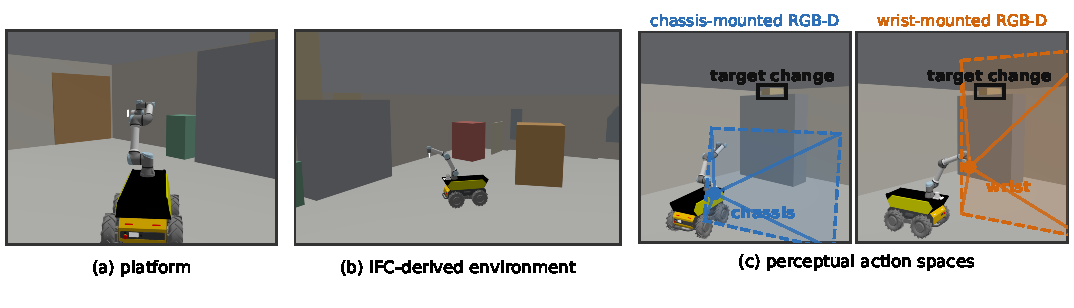
\includegraphics[width=0.74\textwidth]{figures/fig_platform.pdf}
  \caption{The study, in simulation. (a)~A Husky~A300 with a UR5e, carrying a
  chassis RGB-D camera and a lidar on the deck and an identical RGB-D camera at
  the wrist. (b)~Hall~B, clipped from a real Revit IFC export, with the eight
  injected changes. (c)~Admissible observation sets: each sub-panel uses the
  base yaw that aims \emph{its} sensor at the same target, since the arm
  rotates the wrist camera $90^\circ$ off the base heading. Frusta are drawn to
  the target's depth; the change falls outside the chassis frustum and inside
  the wrist one. Renders and frusta come from the evaluation's camera poses.}
  \label{fig:platform}
\end{figure*}

A construction site is not a scene to be mapped once. Between two visits walls
are erected, services are hung, pallets are delivered and consumed, and
formwork is struck; the regions that changed are precisely the regions a
verification system cares about. Robotic capture pipelines are nevertheless
organised predominantly around passive accumulation: a coverage route is
driven, point clouds or images are collected, registered to the model, and
differenced offline~\cite{bosche2010,turkan2012,golparvar2015}. Registration
depends on correspondence between what was observed before and what is observed
now, and large change is exactly the regime in which that correspondence
becomes sparse: the information the robot most requires is the information its
pipeline is least equipped to acquire.

Active perception provides the alternative
framing~\cite{bajcsy1988,aloimonos1988}: sensor placement is treated as a
decision that resolves a specific uncertainty. Applied to an evolving building,
this amounts to asking where to look next in order to determine whether part of
the model still describes reality, which requires answering, in sequence, where
to observe, how to observe, and when sufficient evidence has been gathered.

This paper takes a deliberately narrow first step. Before a planner can choose
among sensing configurations, the set of observations the robot's embodiment
makes available must be characterised. A mobile manipulator can place a camera
almost anywhere in its reachable workspace; a fixed chassis sensor cannot. That
freedom is commonly assumed valuable and seldom measured. Our contributions are
a formulation separating the admissible observation set of an embodiment from
the cost of reaching it; a reproducible IFC-derived benchmark that clips a real
Revit export into a room-scale scene and injects controlled changes labelled by
an observability class describing \emph{why} they are hard to observe; and an
exhaustive sensor-configuration study whose central finding is a distinction we
believe generalises --- embodiment partitions scene changes into those a
configuration cannot observe at all, and those it can observe only at greater
cost.

%%%%%%%%%%%%%%%%%%%%%%%%%%%%%%%%%%%%%%%%%%%%%%%%%%%%%%%%%%%%%%%%%%%%%%%%%%%%%%%%
\section{RELATED WORK}

\textbf{As-built verification} against a building model is well established,
from dimensional compliance checking~\cite{bosche2010} to progress
tracking~\cite{turkan2012,golparvar2015}. Such systems consume data rather than
plan it: the route is set by coverage or an operator, and the verification
objective does not influence where the sensor goes.

\textbf{Active perception} treats sensing as an action to be
planned~\cite{bajcsy1988,aloimonos1988}. Next-best-view methods maximise
expected information for reconstruction~\cite{connolly1985,isler2016} or
exploration~\cite{bircher2016,yamauchi1997}, typically under an unknown-space
objective. Our setting differs: a strong prior exists, and the question
concerns what has \emph{changed}. Mounting the sensor on a manipulator enlarges
the achievable viewpoint set, but the magnitude of that gain is rarely
quantified.

%%%%%%%%%%%%%%%%%%%%%%%%%%%%%%%%%%%%%%%%%%%%%%%%%%%%%%%%%%%%%%%%%%%%%%%%%%%%%%%%
\section{PROBLEM FORMULATION}

Let $M$ denote prior knowledge of the environment, such as a BIM model, a
previous map, or a registered scan, and let $E_t$ denote the unknown physical
state at time $t$. A sensing configuration $q$ consists of a mobile-base
configuration $q_b$ and an arm configuration $q_a$:
\begin{equation}
  q = \left( q_b,\, q_a \right)
\end{equation}
A general active-perception system would select a feasible configuration by
trading the expected task-relevant utility of a future observation against its
acquisition cost:
\begin{equation}
  q^{\ast} = \argmax_{q \in Q}\;
  \bigl[\, U\!\left(q \mid M, B_t\right) - \lambda\, C(q) \,\bigr]
\end{equation}
Here $Q$ is the feasible sensing-action space, $B_t$ denotes the evidence or
belief accumulated so far, $U$ is the expected utility of the observation for
the current task, and $C$ is the cost of acquiring it. The long-term DeltaSeek
objective is to instantiate $U$ using perceptual evidence such as RGB, depth,
point-cloud completeness, registration confidence, or task-specific
uncertainty, and to introduce a stopping rule for deciding when further sensing
is unnecessary.

The present paper deliberately isolates the geometric prerequisite for~(2).
For a scene change or observation target $e$ and sensing configuration $q$, let
$V(e, q) \in [0,1]$ be the visible supporting-surface fraction after range,
frustum, incidence, and occlusion tests. An observation is considered
geometrically admissible when
\begin{equation}
  V(e, q) \;\geq\; \tau_v,
  \qquad \text{with} \quad \tau_v = 0.05
\end{equation}
For sensing embodiment $s$ (chassis or wrist), define the admissible
observation set
\begin{equation}
  Q_e^{\,s} \;=\; \left\{\, q \in Q_s \;:\; V(e,q) \geq \tau_v \,\right\}
\end{equation}
The set $Q_e^{\,s}$ provides the central decomposition studied in this paper.
If $Q_e^{\,s}$ is empty, the target lies outside the sensing capability of
embodiment $s$ and no routing policy can recover it. If $Q_e^{\,s}$ is
nonempty, the observation is feasible and the question becomes how much motion
is required to reach one of its admissible configurations. With start
configuration $q_0$, an idealised acquisition cost is
\begin{equation}
  C_s(e) \;=\; \min_{q \in Q_e^{\,s}} d_{\mathrm{nav}}\!\left(q_0, q\right)
\end{equation}
where $d_{\mathrm{nav}}$ is collision-aware drivable distance; in planned runs
the realised cost is the accumulated route length at which $e$ is first
observed. Fig.~\ref{fig:result} visualises these two quantities directly: the
left panel estimates the size of $Q_e^{\,s}$, the right panel the cost of
reaching it.

%%%%%%%%%%%%%%%%%%%%%%%%%%%%%%%%%%%%%%%%%%%%%%%%%%%%%%%%%%%%%%%%%%%%%%%%%%%%%%%%
\section{BENCHMARK}

\subsection{From IFC to a room-scale scene}

The benchmark derives its geometry from a Revit~2025 IFC2X3~\cite{ifc} export
of a single-storey building, $44.5 \times 19.0 \times 4.5$~m, comprising $133$
products that convert without failure through
IfcOpenShell~\cite{ifcopenshell}. Each product is approximated by a box
oriented in its own placement frame. Orientation is not a refinement: the
export sits on a site grid rotated $0.90^\circ$ from the world axes, and a
world-aligned box expands a $0.203$~m wall to $0.82$~m --- a fourfold error on
the dimension deciding whether the robot fits between two walls.

A storey is an unsuitable unit for studying observation --- one wall entity
spans the full $39$~m of a facade --- so we clip the manifest to a rectangle,
cutting in each element's own frame to preserve the rotation. The resulting
scene, Hall~B (Fig.~\ref{fig:platform}b), measures $7.0 \times 12.5$~m and
contains twelve modelled elements plus two added fit-out units, since the
export has no furniture and both occlusion and height-limited observability
need objects to stand behind or on top of.

\subsection{Observation model}

The visibility term $V(e,q)$ of~(3) is evaluated geometrically rather than from
rendered imagery. An element's surface is sampled, and a sample counts when it
lies within the view frustum, faces the camera within a $75^\circ$ incidence
limit, and is unoccluded. Each change type carries its own supporting surface:
an unmodelled object is supported by seeing the object, a displaced element by
seeing it in its new position or its modelled volume empty. The threshold
$\tau_v = 0.05$ stands in for detector sensitivity. The model assumes perfect
recognition and localisation, so it measures \emph{viewpoint quality} rather
than perception robustness; in exchange it is fast enough to evaluate
exhaustively over $Q_s$, which rendering is not.

\subsection{Acquisition cost}

The distance $d_{\mathrm{nav}}$ of~(5) is a Dijkstra search over an occupancy
grid inflated by the platform's Nav2 footprint ($0.606$~m circumscribed radius,
$0.06$~m resolution). The choice matters: on the storey-scale scene drivable
distance averages $1.8\times$ the straight line and reaches $11\times$, and a
straight-line surrogate would let a robot pass through walls to reach a
viewpoint.

\subsection{Observability classes}

The type of a change describes what moved; it says nothing about whether a
sensor can observe it. We therefore label each change by \emph{why} it is hard
to observe:

\emph{trivial}, a large unmodelled object in open floor space; \emph{height},
above the chassis camera's sightline; \emph{incidence}, resolvable only from an
oblique angle; and \emph{occluded}, in another object's shadow from most base
poses.

Eight changes were hand-placed in Hall~B, two per class, in a committed
scenario rather than sampled, so that each is explainable from geometry and the
study is exactly reproducible. The \emph{trivial} pair is a control: a
configuration that misses it is demonstrably broken.

%%%%%%%%%%%%%%%%%%%%%%%%%%%%%%%%%%%%%%%%%%%%%%%%%%%%%%%%%%%%%%%%%%%%%%%%%%%%%%%%
\section{SENSING CONFIGURATIONS}

The platform is a Clearpath Husky~A300 with an AMP enclosure and a UR5e,
generated from a single \texttt{robot.yaml} so simulation and hardware share
one description. It carries two RGB-D cameras of the \emph{same} model, so the
comparison isolates where a camera is mounted rather than how capable it is.
The \textbf{chassis} embodiment places the camera on the enclosure deck at
$(0.460, 0.000, 0.418)$~m in the base frame, pitched $0.17$~rad down; its pose
is a function of $q_b$ alone. The \textbf{wrist} embodiment is eye-in-hand, its
pose obtained by forward kinematics over the generated description across five
inspection postures $q_a$, verified against the running simulation's transform
tree to machine precision.

The base configurations $q_b$ lie on a $1.0$~m grid of navigable free space
inside the room at four yaw bins $90^\circ$ apart, giving $|Q_b| = 240$
admissible base poses from $60$ positions; both embodiments share this set, so
the comparison is not confounded by base sampling. Each base pose combines with
the five arm postures, so $|Q_{\mathrm{wrist}}| = 1200$ distinct camera poses
while $|Q_{\mathrm{chassis}}| = 240$, the chassis camera being invariant to
$q_a$. In the \emph{both} configuration an element is observed if either sensor
observes it.

\begin{figure}[t]
  \centering
  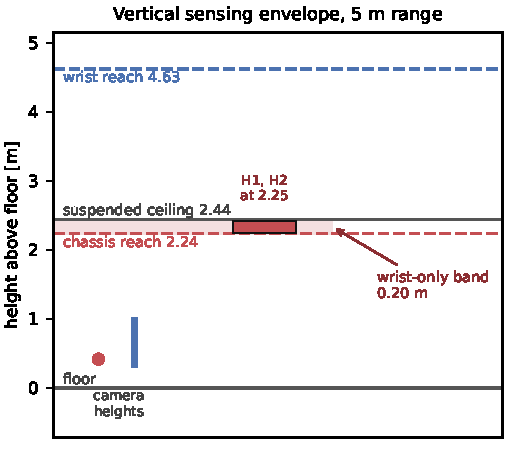
\includegraphics[width=0.78\columnwidth]{figures/fig_reach.pdf}
  \caption{Why exactly two changes admit no chassis viewpoint. At the $5$~m
  range limit the chassis camera reaches $2.24$~m and the wrist camera
  $4.63$~m. The ceiling begins at $2.44$~m, leaving a wrist-only band $0.20$~m
  tall, in which the two \emph{height} changes sit at $2.25$~m. Both reaches
  are closed-form, and agree with a numeric sweep to $3$~mm.}
  \label{fig:reach}
\end{figure}

%%%%%%%%%%%%%%%%%%%%%%%%%%%%%%%%%%%%%%%%%%%%%%%%%%%%%%%%%%%%%%%%%%%%%%%%%%%%%%%%
\section{RESULTS}

\begin{figure*}[t]
  \centering
  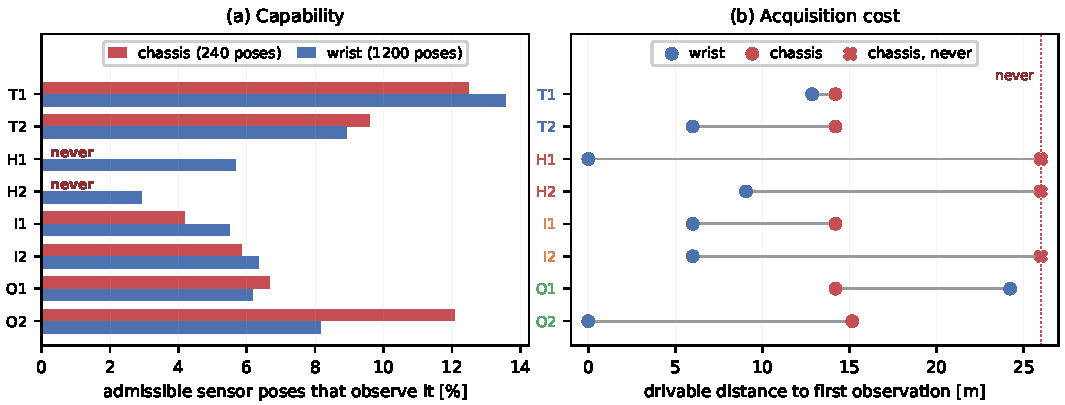
\includegraphics[width=0.52\textwidth]{figures/fig_result.pdf}
  \caption{(a)~Capability: $|Q_e^{\,s}|$ as a share of admissible sensor poses
  for each change; two changes satisfy $Q_e^{\,\mathrm{chassis}} = \emptyset$.
  (b)~Acquisition cost: drivable distance to first observation under a $25$~m
  budget.}
  \label{fig:result}
\end{figure*}

\begin{table}[t]
  \caption{Changes observed, by observability class}
  \label{tab:main}
  \centering
  \begin{tabular}{lccc}
    \toprule
    Class & chassis & wrist & both \\
    \midrule
    trivial    & 2/2          & 2/2 & 2/2 \\
    height     & \textbf{0/2} & 2/2 & 2/2 \\
    incidence  & 1/2          & 2/2 & 2/2 \\
    occluded   & 2/2          & 2/2 & 2/2 \\
    \midrule
    all        & 5/8          & 8/8 & 8/8 \\
    \bottomrule
  \end{tabular}
\end{table}

\subsection{Capability: the structure of $Q_e^{\,s}$}

Table~\ref{tab:main} reports what each configuration observed within a $25$~m
budget; Fig.~\ref{fig:result}(a) reports the underlying capability.

The result of interest is not the $5/8$ figure. A single planned run conflates
$Q_e^{\,s} = \emptyset$ with the case in which one route failed to reach an
admissible pose, so we separate the two by evaluating $V(e,q)$ at every
$q \in Q_s$. For two changes --- both of class \emph{height} ---
$Q_e^{\,\mathrm{chassis}}$ is empty, at zero visible fraction across all $240$
chassis poses; this is a property of the embodiment. A third change that the
chassis-only run missed satisfies $|Q_e^{\,\mathrm{chassis}}| = 14$: the
planner did not visit an admissible pose within budget, which is a routing
outcome, not evidence for the manipulator. The distinction is not merely
formal --- repositioning the arm on the deck during development moved the
planned chassis result from $6/8$ to $5/8$ while the capability figure did not
move at all.

Fig.~\ref{fig:reach} explains why only the \emph{height} class produces an
empty admissible set. For a camera of pitch $p$ at height $h$ with vertical
field of view $v$, the highest world point inside its frustum at range $r$ is
$h + r\left(\cos p \tan \tfrac{v}{2} - \sin p\right)$, with no yaw term: yaw
rotates about the vertical axis and cannot alter the vertical extent. At
$r = 5$~m this gives $2.24$~m for the chassis camera and $4.63$~m for the
wrist, against a ceiling at $2.44$~m. The wrist-only band is therefore
$0.20$~m tall, and the two \emph{height} changes were placed within it at
$2.25$~m.

\subsection{Acquisition cost: $C_s(e)$ where both embodiments succeed}

The \emph{occluded} and \emph{incidence} pairs were designed to require the
manipulator and did not. The crate behind the pallet stack satisfies
$|Q_e^{\,\mathrm{chassis}}| = 16$ of $240$ --- hidden from $93\%$ of chassis
poses, as intended --- but a planner needs only one of those sixteen. Where
both embodiments succeed the difference appears in $C_s(e)$, not in detections
(Fig.~\ref{fig:result}(b)): the median drivable distance to first observation
is $6.0$~m for the wrist and $14.2$~m for the chassis, a factor of $2.4$.
Occlusion, the intuitive case for a manipulator, is in this environment a
routing cost paid in metres rather than a sensing limit.

%%%%%%%%%%%%%%%%%%%%%%%%%%%%%%%%%%%%%%%%%%%%%%%%%%%%%%%%%%%%%%%%%%%%%%%%%%%%%%%%
\section{DISCUSSION}

Two effects follow, and an active-perception system must treat them
differently. \textbf{Sensing capability} is binary and fixed by embodiment:
when $Q_e^{\,s} = \emptyset$ no planning policy recovers the change, and the
utility term $U$ of~(2) is identically zero over $Q_s$. \textbf{Acquisition
cost} is continuous and fixed by the environment: the information exists, and
the question is the value of $C_s(e)$. This is where viewpoint planning has
leverage, and where the $6.0$~m against $14.2$~m difference lives. Conflating
the two is easy, since a single run reports only ``observed'' or ``not
observed'' and an expensive change is then indistinguishable from an impossible
one.

The capability boundary is also a design variable: the wrist-only band in
Hall~B is $0.20$~m because the chassis camera sits at $0.418$~m pitched
$0.17$~rad down, levelling it shrinks the band toward zero, and a taller space
widens it. The useful output is therefore not the claim that the manipulator is
worth two changes, but a method for locating that boundary before a platform
design is committed.

\section{LIMITATIONS AND FUTURE WORK}

The study is narrow: one room, one ceiling height, eight changes. The $0.20$~m
band is a property of this geometry, and a trend requires rooms of differing
height. Detection is geometric --- no detector, no renderer, no noise --- so
the reported quantities describe viewpoint quality, not whether a perception
stack would recover the change. Elements are boxes, discarding the $48$ opening
entities in the source model, so Hall~B is a sealed room the robot must be
spawned inside. The height margin is thin: the \emph{height} pair clears the
chassis ceiling by $11.8$~mm, so levelling or raising that camera would close
the gap --- the design-variable observation above, restated as a caution.
Finally, the framework does not yet answer its third question: deciding
\emph{when} enough evidence has been gathered requires a graded belief $B_t$
and a stopping rule, not binary detection.

%%%%%%%%%%%%%%%%%%%%%%%%%%%%%%%%%%%%%%%%%%%%%%%%%%%%%%%%%%%%%%%%%%%%%%%%%%%%%%%%
\section{CONCLUSION}

DeltaSeek is a first step toward robots that plan perception in environments
that do not hold still. We formalised the contribution of a mobile
manipulator's embodiment as the structure of the admissible observation set
$Q_e^{\,s}$ and the cost $C_s(e)$ of reaching it, and measured both on an
IFC-derived benchmark. The answer is sharper and smaller than the usual
assumption: two of eight changes lie outside the chassis camera's admissible
set entirely, and the rest cost roughly $2.4\times$ the travel. A robot that is
one day to decide when it has seen enough must first distinguish a view it
cannot obtain from one it has not yet paid for.

%%%%%%%%%%%%%%%%%%%%%%%%%%%%%%%%%%%%%%%%%%%%%%%%%%%%%%%%%%%%%%%%%%%%%%%%%%%%%%%%
\begin{thebibliography}{99}
\setlength{\itemsep}{-1.5pt}

\bibitem{bosche2010}
F.~Bosch\'e, ``Automated recognition of 3D CAD model objects in laser scans and
calculation of as-built dimensions for dimensional compliance control in
construction,'' \emph{Advanced Engineering Informatics}, vol.~24, no.~1,
pp.~107--118, 2010.

\bibitem{turkan2012}
Y.~Turkan, F.~Bosch\'e, C.~T.~Haas, and R.~Haas, ``Automated progress tracking
using 4D schedule and 3D sensing technologies,'' \emph{Automation in
Construction}, vol.~22, pp.~414--421, 2012.

\bibitem{golparvar2015}
M.~Golparvar-Fard, F.~Pe\~na-Mora, and S.~Savarese, ``Automated progress
monitoring using unordered daily construction photographs and IFC-based
building information models,'' \emph{Journal of Computing in Civil
Engineering}, vol.~29, no.~1, 2015.

\bibitem{bajcsy1988}
R.~Bajcsy, ``Active perception,'' \emph{Proceedings of the IEEE}, vol.~76,
no.~8, pp.~966--1005, 1988.

\bibitem{aloimonos1988}
J.~Aloimonos, I.~Weiss, and A.~Bandyopadhyay, ``Active vision,''
\emph{International Journal of Computer Vision}, vol.~1, no.~4, pp.~333--356,
1988.

\bibitem{connolly1985}
C.~Connolly, ``The determination of next best views,'' in \emph{Proc. IEEE Int.
Conf. Robotics and Automation (ICRA)}, 1985, pp.~432--435.

\bibitem{isler2016}
S.~Isler, R.~Sabzevari, J.~Delmerico, and D.~Scaramuzza, ``An information gain
formulation for active volumetric 3D reconstruction,'' in \emph{Proc. IEEE Int.
Conf. Robotics and Automation (ICRA)}, 2016, pp.~3477--3484.

\bibitem{bircher2016}
A.~Bircher, M.~Kamel, K.~Alexis, H.~Oleynikova, and R.~Siegwart, ``Receding
horizon `next-best-view' planner for 3D exploration,'' in \emph{Proc. IEEE Int.
Conf. Robotics and Automation (ICRA)}, 2016, pp.~1462--1468.

\bibitem{yamauchi1997}
B.~Yamauchi, ``A frontier-based approach for autonomous exploration,'' in
\emph{Proc. IEEE Int. Symp. Computational Intelligence in Robotics and
Automation (CIRA)}, 1997, pp.~146--151.

\bibitem{ifc}
ISO 16739-1:2018, \emph{Industry Foundation Classes (IFC) for data sharing},
ISO, Geneva, 2018.

\bibitem{ifcopenshell}
IfcOpenShell IFC toolkit and geometry engine. [Online]. Available:
\url{https://ifcopenshell.org}

\end{thebibliography}

\end{document}
